% Knowledge and Information Systems (Springer) -- regular research article
% Springer Nature authoring template (sn-jnl) with sn-basic numbered references.
% Compile: pdflatex; bibtex; pdflatex x2
\documentclass[pdflatex,sn-basic,Numbered]{sn-jnl}

\usepackage{amsmath,amssymb,amsthm}
\usepackage{booktabs}
\usepackage{array}
\usepackage{tabularx}
\usepackage{graphicx}
\usepackage{xcolor}
\usepackage{xurl}
\usepackage{textcomp}
\usepackage{manyfoot}

\graphicspath{{figures/}}
\setlength{\emergencystretch}{2em}

\begin{document}

\title[Region-Specific Incremental Feature Menus]{Region-Specific Incremental Feature Menus for Progressive Feature Revelation}

\author*[1]{\fnm{Hoa Dinh} \sur{Nguyen}}\email{hoand@ptit.edu.vn}

\affil*[1]{\orgname{Posts and Telecommunications Institute of Technology}, \orgaddress{\city{Hanoi}, \country{Vietnam}}}

\abstract{When covariates must be acquired under a budget, a predictor should be useful before the full feature vector is observed. This paper treats that setting as knowledge discovery: the object to be mined is a collection of region-specific ordered feature menus---inspectable lists of which measurements to obtain next in each region of the input space.

The method partitions the training inputs, runs forward stepwise selection with Bayesian information criterion (BIC) stopping inside each region, and stores nested prefix least-squares models. At test time a query is assigned to regions and features are revealed along the local menu. Performance is scored by an anytime root-mean-square error (RMSE) curve. A nested training check compares regional and global RMSE at a small budget and deploys only the cheaper policy.

On computed tomography (CT) slice localization (\(n\) up to \(5.35\times 10^4\), \(p=384\)) and superconductivity prediction (\(n\approx 2.1\times 10^4\), \(p=81\)), region menus reduce progressive RMSE relative to global stepwise. Early entries differ across regions and correspond to distinct histogram channels (CT) and elemental-property families (superconductivity). Localized Lasso--LARS menus and a local residual-greedy policy remain weaker at early budgets. Mixed synthetics and a weak-signal control show that a single global menu can suffice when mechanisms are homogeneous or signal is scarce; the nested check recovers that scope from training data.}

\keywords{feature selection, knowledge discovery, anytime prediction, local models, data mining, progressive feature revelation}

\maketitle

\noindent Corresponding author. ORCID: \url{https://orcid.org/0009-0004-1708-9248}.

\noindent\textbf{Acknowledgments.} The author has no acknowledgments to report.

\section{Introduction}
\label{sec:intro}

Classical supervised regression is usually formulated under a complete observation assumption: for a query \(\mathbf{x}_q\in\mathbb{R}^p\), where \(p\) denotes the feature dimension, all coordinates are available before prediction. In knowledge-discovery and data-engineering settings that assumption is often unrealistic. Measurements may be costly, streamed, or revealed on demand: only a subset of imaging descriptors may be computed under a latency budget; additional spectral or physicochemical variables incur cost; sensors come online asynchronously. Prediction must then be useful before the full feature vector is known.

This induces a progressive feature revelation (or anytime acquisition) problem \cite{ma2019,covert2023}: features are disclosed one by one according to an acquisition order \(\pi\), and after budget \(b\) the learner may use only the first \(b\) revealed coordinates. The natural performance object is not a single test root-mean-square error (RMSE), but a curve of error versus budget. An acquisition policy is valuable if it reduces error quickly at small \(b\), not only if it eventually matches a full-feature model. From a knowledge-systems perspective, the policy itself is the knowledge artifact: an ordered list of what to measure next.

A simple and widely used family of policies learns one global feature order---for example by ranking absolute correlations with the response \cite{guyon2003}, by forward stepwise regression, by least absolute shrinkage and selection operator (Lasso) / least-angle regression (LARS) regularization paths \cite{tibshirani1996,efron2004}, or by streamwise procedures such as \(\alpha\)-investing and variance inflation factor (VIF) regression \cite{zhou2006,foster2008,lin2011}. The same order is then applied to every query. Global orders are easy to interpret and often strong when the regression mechanism is approximately homogeneous. Their weakness is structural: they ignore regional heterogeneity. Different parts of the input space may depend on different covariates, so the feature that is most useful on average need not be the feature that is most useful for this query.

The central idea of this paper is that acquisition knowledge should be piecewise, not global. If the input space can be partitioned into regions with relatively stable local relevance patterns, then an ordered feature menu can be maintained for each region. A query is first localized to a region (or a soft combination of regions); subsequent acquisitions are guided by that menu; and predictions are produced by nested models trained on menu prefixes. In effect, a single acquisition schedule is replaced by a mixture of schedules. Because each regional menu can be stored, inspected, and executed cheaply at test time, the resulting representation is local feature knowledge in the ordinary data-mining sense: compact, auditable, and reusable.

This idea sits between two classical traditions. On one side, local learning adapts the regression fit to a neighborhood of the query \cite{atkeson1997,cleveland1988}, but typically assumes that the neighborhood already has access to the same full feature set. On the other side, feature selection produces sparse supports or ordered lists \cite{guyon2003}, but usually one list for the entire population. Progressive revelation needs both ingredients: locality in which features matter, and incrementality in when they are acquired. A computationally light compromise is obtained via region-specific menus---constant menus within regions, rather than a fully instance-adaptive acquisition policy \cite{ma2019,covert2023}---while interpretability and scalability to tens of thousands of samples and hundreds of features are retained.

``Just cluster and select'' is insufficient as a scientific contribution unless carefully formulated, for several reasons:
\begin{enumerate}
  \item \textbf{Objective mismatch.} Feature selection is usually tuned for full-feature risk (or model sparsity). Accuracy of the nested-model path at intermediate budgets is required under progressive revelation. Even when a good final support is eventually found, poor early features may still be acquired.
  \item \textbf{Partition quality.} Regions formed from a feature matrix \(\mathbf{X}\) alone may not be aligned with changes in the regression mechanism. Conversely, partitions that use a response vector \(\mathbf{y}\) at training time must still be usable at test time from \(\mathbf{X}\) only.
  \item \textbf{Sample fragmentation.} Per-region sample size is reduced when data are split into regions, and selection can be destabilized, especially when \(p\) is large. Usefulness of the method under this bias--variance tension must be retained.
  \item \textbf{Evaluation discipline.} Claims about progressive revelation must be tested with anytime curves and with negative controls: weak-signal data and regimes where global selection is already near-optimal.
\end{enumerate}

This study makes the following three contributions, sized for a knowledge-discovery rather than a general learning-theory claim:
\begin{enumerate}
  \item \textbf{Knowledge representation.} Progressive feature revelation is formalized, and region-specific incremental feature menus are defined as piecewise-constant acquisition knowledge: one ordered list per region, with nested prefix predictors for partial-information prediction.
  \item \textbf{Mining procedure.} A two-stage pipeline partitions the inputs (hard or soft assignment; residual-aware clustering), mines a forward-stepwise BIC menu in each region with nested OLS prefix models, and then chooses from training data whether to deploy those menus or a single global stepwise menu.
  \item \textbf{Evaluation protocol with bounded claims.} Menus are scored by anytime RMSE, named as domain knowledge, compared with localized Lasso--LARS and with local residual-greedy acquisition, and read as a measurement budget. Mixed and weak-signal controls, plus the nested pre-test, delimit when a global menu remains sufficient.
\end{enumerate}

The remainder of the paper is as follows. Related work and gaps are reviewed in Section~\ref{sec:related}. The proposed method is presented in Section~\ref{sec:method}. Experimental results are presented in Section~\ref{sec:experiments}. Implications and limitations are discussed in Section~\ref{sec:discussion}. Conclusions are given in Section~\ref{sec:conclusion}.

\section{Related work}
\label{sec:related}

Feature selection is a core knowledge-discovery task: identify a compact, interpretable subset (or ranking) of variables that supports prediction and explanation \cite{guyon2003,li2017kais,bolon2013kais}. Filter, wrapper, and embedded methods remain the standard taxonomy. Forward stepwise regression is a greedy path method; Lasso and LARS provide regularization paths whose entry order can also be read as a ranking \cite{tibshirani1996,efron2004}. Controlled synthetic studies have long been used to stress-test selectors under irrelevance, redundancy, and small \(n/p\) \cite{bolon2013kais}. Greedy selectors typically return one solution, even when several statistically equivalent supports exist \cite{borboudakis2021}; regional menus make a related point in a different direction, by retaining several ordered lists that are specialized to subpopulations rather than alternative global supports.

Streamwise and online feature selection consider candidates sequentially and control overfitting via adaptive thresholds, notably \(\alpha\)-investing and VIF regression \cite{zhou2006,foster2008,lin2011}. Online streaming feature selection further addresses features that arrive over time \cite{wu2013,zhou2017kbs}. These methods usually produce one ordered support for the whole training distribution. Progressive revelation exposes a second axis of difficulty: the order that is optimal globally may be suboptimal locally. Incremental selectors are reused here as menu constructors inside regions, and they are evaluated by anytime error, not only by final support quality.

Clusterwise regression and mixture-of-experts models allow different linear predictors in different latent groups \cite{desarbo1988,jordan1994}. Sparse mixtures and localized Lasso learn supports that vary across components, samples, or clusters \cite{chamroukhi2019,yamada2017,dimari2023,binder2012}. That literature typically optimizes full-observation risk or subgroup interpretability, not an acquisition schedule under partial observation. Localized Lasso--LARS menus are therefore re-scored in Section~\ref{sec:experiments} under the same nested anytime protocol.

Locally weighted and memory-based regression adapt the fit to a neighbourhood of the query \cite{atkeson1997,cleveland1988,birattari1998,schaal1998,vijayakumar2005}, but they assume that the same coordinates are already observed. They do not, by themselves, choose which feature to acquire next.

Cost-sensitive feature selection incorporates measurement costs when forming a compact subset \cite{zhou2016kbs}, yet the support is typically global and is scored by full-observation accuracy. Fully instance-adaptive policies choose the next unobserved coordinate using conditional mutual information or reinforcement learning \cite{ma2019,covert2023}. Those methods can be powerful but are heavy to deploy and hard to audit. A classical stand-in---local residual-greedy acquisition in the already observed coordinates---is evaluated in Section~\ref{sec:experiments}. Region-specific menus occupy the middle ground: piecewise-constant acquisition knowledge, cheap to store and inspect, without solving a full dynamic acquisition Markov decision process.

Synthesizing the above, three gaps motivate this work:
\begin{enumerate}
  \item Anytime evaluation is underused in localized sparse regression and knowledge-discovery papers, which often report only full-feature metrics.
  \item Global incremental selectors ignore regional relevance shifts, yet are still the default construction for ordered acquisition lists.
  \item Fully adaptive acquisition policies are heavy; a middle ground---region-constant menus as stored local knowledge, with soft assignment---has not been systematically compared, under anytime RMSE, both with global menus and with a classical instance-adaptive greedy rule.
\end{enumerate}

That middle ground is targeted in this work. Region-specific incremental menus are studied as mined acquisition knowledge. The approach is validated with both positive heterogeneous cases and mixed or negative controls.

\section{Proposed method}
\label{sec:method}

The overall pipeline is summarized in Fig.~\ref{fig:method}: the input space is partitioned, a forward-stepwise BIC menu is built in each region, nested prefix OLS models are fitted, and at test time a query is assigned to regions before features are acquired along the local menu up to budget~$b$.

\begin{figure}[t]
\centering
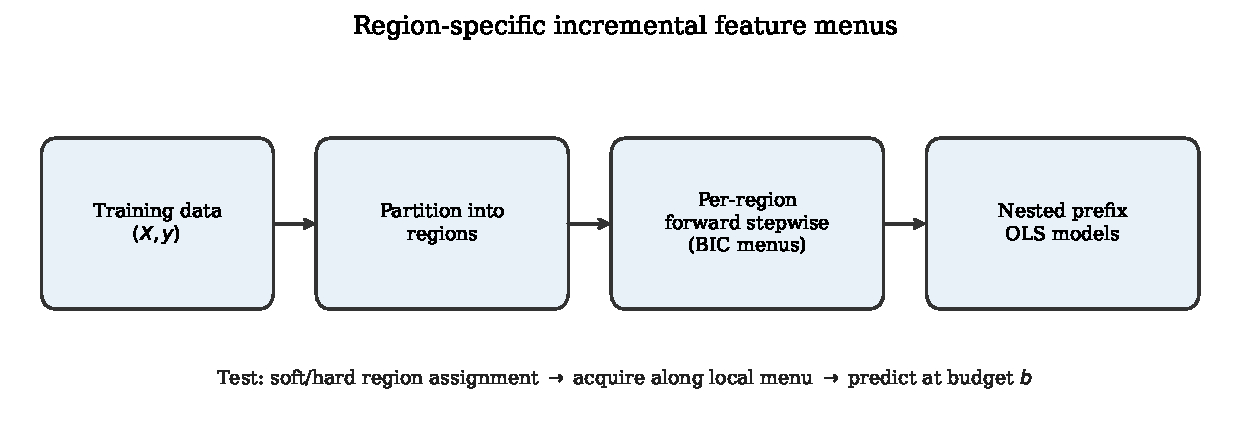
\includegraphics[width=\textwidth]{fig1_method_overview.pdf}
\caption{Overview of region-specific incremental feature menus. Training partitions the input space, builds a forward-stepwise Bayesian information criterion (BIC) menu in each region, and fits nested prefix ordinary least-squares (OLS) models. At test time, a query is assigned to regions and features are acquired along the local menu up to budget~$b$}
\label{fig:method}
\end{figure}

\subsection{Progressive feature revelation}

Vectors and matrices are written in bold; scalars are not. Let the training sample be \(\mathcal{D}=\{(\mathbf{x}_i,y_i)\}_{i=1}^n\), where \(n\) is the number of training samples, each feature vector \(\mathbf{x}_i\in\mathbb{R}^p\) has dimension \(p\), and \(y_i\in\mathbb{R}\) is the scalar response. Write \(\mathbf{X}\in\mathbb{R}^{n\times p}\) for the feature matrix with rows \(\mathbf{x}_i^\top\) and \(\mathbf{y}=(y_1,\ldots,y_n)^\top\in\mathbb{R}^n\) for the response vector. A (deterministic) acquisition order is a sequence \(\pi=(j_1,\ldots,j_m)\) of distinct feature indices, with menu length \(m\le p\). After budget \(b\in\{0,\ldots,m\}\), only coordinates in the prefix
\[
S_b(\pi)=\{j_1,\ldots,j_b\}
\]
may be used, with the empty prefix \(S_0=\emptyset\). A progressive predictor is a family \(\{\hat f_b\}_{b=0}^m\) where \(\hat f_b\) depends on a query \(\mathbf{x}\) only through coordinates in \(S_b(\pi)\). Performance is summarized by the anytime RMSE curve
\[
\mathrm{RMSE}(b)=\Bigl(\tfrac{1}{n_{\mathrm{te}}}\sum_{q=1}^{n_{\mathrm{te}}}\bigl(y_q-\hat f_b(\mathbf{x}_q)\bigr)^2\Bigr)^{1/2},
\]
where \(n_{\mathrm{te}}\) is the number of test samples and \((\mathbf{x}_q,y_q)\) denotes the \(q\)-th test pair. The goal is to learn orders and prefix models that make \(\mathrm{RMSE}(b)\) small for small and moderate \(b\), not only for \(b=m\).

\subsection{Region-specific menus: overview}

\(R\) regions are maintained, indexed by \(r\in\{1,\ldots,R\}\). Region \(r\) has:
\begin{itemize}
  \item a center \(\mathbf{c}_r\in\mathbb{R}^p\) used for assignment from \(\mathbf{X}\);
  \item a menu \(\pi^{(r)}=(j^{(r)}_1,\ldots,j^{(r)}_{m_r})\) of length \(m_r\);
  \item nested prefix models \(\{\hat f^{(r)}_b\}_{b=0}^{m_r}\).
\end{itemize}

Training proceeds in three stages: (i) partition training points into regions; (ii) run incremental feature selection inside each region to obtain \(\pi^{(r)}\); (iii) fit nested OLS models on menu prefixes. A fourth, optional stage (Section~\ref{sec:method-pretest}) compares this regional fit with a one-region global menu on held-out training data and deploys only the cheaper policy. At test time, a query is assigned to regions, a menu is chosen (or soft-combined), and predictions are read from the corresponding prefix model(s).

\subsection{Partitioning}

All partitioning operates after column-wise standardization of \(\mathbf{X}\) fitted on the training fold. Let \(\mathbf{X}^{\mathrm{sc}}\in\mathbb{R}^{n\times p}\) denote the standardized feature matrix. When the response or residual channel is used, that one-dimensional vector is standardized separately to zero mean and unit variance, writing \(\mathbf{y}^{\mathrm{sc}}\in\mathbb{R}^n\) and \(\hat{\mathbf{r}}^{\mathrm{sc}}\in\mathbb{R}^n\). Thus the residual-aware and response-augmented schemes do not mix quantities on incompatible scales before clustering.

\subsubsection{\texorpdfstring{\(k\)}{k}-means on \texorpdfstring{\(\mathbf{X}\)}{X} (\texttt{kmeans})}
\(\mathbf{X}^{\mathrm{sc}}\) is clustered into \(R\) groups. Region centers used at test time are the empirical means of \(\mathbf{X}^{\mathrm{sc}}\) within each cluster.

\subsubsection{Residual-aware clustering (\texttt{residual})}
A global linear model is fitted \(\hat{\mathbf{y}} = \mathbf{X}^{\mathrm{sc}}\hat{\boldsymbol{\beta}}\), and the residual \(\hat{\mathbf{r}} = \mathbf{y}-\hat{\mathbf{y}}\) is standardized to \(\hat{\mathbf{r}}^{\mathrm{sc}}\). \(k\)-means is run on the rows of \([\,\mathbf{X}^{\mathrm{sc}},\, w\hat{\mathbf{r}}^{\mathrm{sc}}\,]\). The extra coordinate separates points that are nearby in \(\mathbf{X}\) but systematically under- or over-predicted by the global fit. After clustering, only \(\mathbf{X}^{\mathrm{sc}}\)-means are stored, so a test query is assigned from \(\mathbf{x}^{\mathrm{sc}}\) alone: the residual channel shapes the training partition without test-time leakage.

\subsubsection{Response-augmented clustering (\texttt{xy})}
The same construction with \(\mathbf{y}^{\mathrm{sc}}\) in place of \(\hat{\mathbf{r}}^{\mathrm{sc}}\). Main experiments use residual clustering.

\subsubsection{Small-region repair}
If a cluster contains fewer than \(n_{\min}\) points, where \(n_{\min}\) is a minimum region-size threshold, its members are reassigned to the nearest sufficiently large region in \(\mathbf{X}^{\mathrm{sc}}\)-space, and region indices are compacted. This mitigates unstable menus in tiny fragments.

\subsection{Per-region incremental selection}

Within region \(r\), let \(\mathcal{D}_r\) be the local sample of size \(n_r\). The menu \(\pi^{(r)}\) is constructed by forward stepwise regression with BIC stopping.

The procedure is started from the intercept-only model. At step \(t\), among unused features, the index that most reduces residual sum of squares (RSS) when added to the current model is selected. The addition is accepted only if BIC decreases:
\[
\mathrm{BIC}= n_r\log(\mathrm{RSS}/n_r) + k\log n_r,
\]
where \(k\) counts free parameters (intercept plus selected slopes). Iteration stops when no candidate improves BIC, or when a cap \(m_{\max}\) on menu length is reached.

\subsubsection{Scalable update}
Rather than refitting OLS for every candidate at every step, an orthonormal basis of the current model span is maintained (starting from a normalized intercept column) and candidates are residualized against that basis. The RSS reduction of adding a residualized candidate \(\mathbf{z}\) equals \((\mathbf{z}^\top \mathbf{e})^2/\|\mathbf{z}\|_2^2\) for current residual vector \(\mathbf{e}\). After accepting a feature, the basis and all candidate residuals are updated by a single rank-one orthogonalization. This yields an \(O(n_r p_{\mathrm{cand}})\) cost per step, where \(p_{\mathrm{cand}}\) is the number of candidate features under consideration, and matches the exact forward-stepwise RSS criterion under full column rank.

\subsubsection{Optional screening}
When \(p\) is large, candidates may first be restricted to the top \(p_{\mathrm{screen}}\) features by absolute Pearson correlation with \(\mathbf{y}\) inside the region. Screening is a computational device; the menu order among survivors is still determined by stepwise BIC.

\subsubsection{Why forward stepwise for menus}
Under the same residual/soft regional scaffold, forward stepwise, VIF regression with \(\alpha\)-investing \cite{lin2011}, and Lasso-LARS path entry orders \cite{efron2004} were compared. Forward stepwise consistently produced competitive or superior early-budget progressive RMSE and typically sparser menus. VIF was competitive but sometimes over-selected; Lasso-LARS often yielded weaker low-budget acquisition orders despite reasonable final supports. Forward stepwise is therefore fixed as the primary menu constructor.

\subsection{Nested prefix models}

Given menu \(\pi^{(r)}\), for each budget \(b\) the design that uses an intercept and features \(\pi^{(r)}_{1:b}\) is defined. OLS is fitted on \(\mathcal{D}_r\) to obtain \(\hat f^{(r)}_b\). Budget \(b=0\) is the regional mean response. These nested models ensure that evaluation at budget \(b\) uses a predictor trained only on the first \(b\) menu features---not a masked version of a full-support model, which would be optimistically biased for progressive revelation.

\subsection{Assignment and prediction at test time}

For a standardized query \(\mathbf{x}^{\mathrm{sc}}\), the squared Euclidean assignment distance is defined as \(d_r(\mathbf{x})=\|\mathbf{x}^{\mathrm{sc}}-\mathbf{c}_r\|_2^2\).

\subsubsection{Hard assignment}
Let \(\hat r(\mathbf{x})=\arg\min_r d_r(\mathbf{x})\). Features are acquired along \(\pi^{(\hat r)}\) and prediction is performed with \(\hat f^{(\hat r)}_b\).

\subsubsection{Soft assignment}
Weights are defined by
\[
w_r(\mathbf{x})\propto \exp\bigl(-d_r(\mathbf{x})/T\bigr),
\]
normalized over \(r\), with temperature \(T>0\). The (scalar) prediction at budget \(b\) is
\[
\hat y(\mathbf{x})=\sum_{r=1}^R w_r(\mathbf{x})\,\hat f^{(r)}_{b_r}(\mathbf{x}),
\]
where \(b_r=\min\{b, m_r\}\) uses each region's own prefix length. Acquisitions follow the primary region \(\arg\max_r w_r(\mathbf{x})\).

\subsection{Choosing regional versus global menus}
\label{sec:method-pretest}
The pipeline above always returns \(R\) menus when \(R>1\). Whether those menus should be deployed, rather than a single global stepwise menu, is a separate knowledge-use decision. It is made from the training sample only.

Let \(\mathcal{D}_{\mathrm{fit}}\) and \(\mathcal{D}_{\mathrm{val}}\) be a random split of the training fold (80\%/20\% in the experiments). Fit the regional residual/soft pipeline and a one-region forward-stepwise menu on \(\mathcal{D}_{\mathrm{fit}}\). Score both by RMSE at a small operating budget \(b^\star\) on \(\mathcal{D}_{\mathrm{val}}\) (\(b^\star=5\) in the reported tables). Refit the cheaper policy on the full training fold. The test fold is never used to choose. Menu-overlap and training BIC of the prefix mixture are cheaper statistics but are not the recommended rule (Section~\ref{sec:when}). The pre-test chooses between the design \(R\) and \(R=1\); it does not search over the integer \(R\).

\subsection{Complexity and implementation profile}

Let \(m\le m_{\max}\) be the final menu length and \(p_{\mathrm{cand}}\) the number of stepwise candidates after screening. Per region, selection costs \(O(m\, n_r p_{\mathrm{cand}})\) with QR factorization updates. Prefix fitting is \(O(m n_r m^2)\) in a naive implementation and is negligible for the moderate \(m\) used here (\(m_{\max}\approx 20\)--\(30\)). Soft prediction is \(O(R p)\) for assignment weights plus \(O(R b)\) for prefix evaluation. The method is therefore practical for \(n\sim 10^4\)--\(10^5\) and \(p\sim 10^2\)--\(10^3\) with screening, as implied by the modular stages in Fig.~\ref{fig:method}.

\section{Experimental results}
\label{sec:experiments}

\subsection{Experimental protocol}

Unless noted otherwise, each dataset is randomly split into training and test folds (typically 75\%/25\% or 70\%/30\%). Feature standardization is fit on the training fold only and applied to the test fold. Progressive RMSE is computed on the test set for budgets \(b=0,1,\ldots,b_{\max}\), where \(b_{\max}\) is the maximum menu length among compared methods (capped by \(m_{\max}\)). For very large test sets, up to 5{,}000 test points are subsampled for scoring while large training sets are retained, so that training reflects large-\(n\) behavior.

All methods share the same splits and preprocessing. Region methods use residual-aware partitioning with soft assignment unless stated, and forward stepwise with BIC stopping as the primary menu constructor. Hyperparameters are not re-optimized at each budget. The nested regional-versus-global pre-test of Section~\ref{sec:method-pretest} is reported in Table~\ref{tab:when}.

\subsubsection{How parameter values are obtained}
Most operating choices are fixed by design or by a simple size-dependent rule rather than by exhaustive cross-validation, so that reported gains are not an artifact of per-dataset oracle tuning. Soft-assignment temperature is held at \(T=1\) after light exploratory checks, and the residual/response augmentation weight is likewise fixed at \(w=1\) (one standardized residual or response unit). The selector itself (forward stepwise with BIC) was chosen from the comparative study in Section~\ref{sec:method} and is then held fixed across datasets. The remaining knobs---number of regions \(R\), minimum region size \(n_{\min}\), menu-length cap \(m_{\max}\), and optional screening width---are set from \(n\) and \(p\) as follows.

\subsubsection{Scaling with \texorpdfstring{\(n\)}{n} and \texorpdfstring{\(p\)}{p}}
The number of regions is chosen by sample-size and problem regime: \(R=4\) is used on the large-\(n\) heterogeneous tasks (CT slices and superconductivity), whereas \(R=3\) is used when samples are scarce relative to dimensionality (tecator), on the weak-signal control (topo\_2\_1), and on the hard synthetic generator whose planted structure has three centers. The minimum region size is set by the rule
\[
n_{\min}=\max\bigl\{40,\,\min\{200,\,\lfloor n_{\mathrm{train}}/(5R)\rfloor\}\bigr\},
\]
so that \(n_{\min}\) grows with training sample size but is bounded below by 40 and above by 200. Consequently, larger CT and superconductivity runs admit larger repaired regions, while tecator remains constrained by its small \(n\). The menu-length cap is \(m_{\max}=25\) on CT slices, superconductivity, topo\_2\_1, and the synthetics; it is reduced to \(m_{\max}=20\) on tecator to limit over-selection under high \(p\)/low \(n\). Actual menu lengths are shorter whenever BIC stops earlier, and the evaluation horizon \(b_{\max}\) is taken as the longest realized menu among compared methods (still capped by \(m_{\max}\)). When \(p>120\), candidates are first restricted by absolute Pearson correlation inside each region to a screen of width \(\min\{p,\max\{100,20\,m_{\max}\}\}\); thus screening is active on CT slices (\(p=384\)), topo\_2\_1 (\(p=266\)), and the synthetics (\(p\in\{1000,2000\}\)), but not on superconductivity (\(p=81\)), and is only lightly binding on tecator (\(p=124\)). In short, \(R\) and \(n_{\min}\) adapt primarily to \(n\), while \(m_{\max}\) and screening width adapt primarily to the \(p\) (and \(p/n\)) regime.

\subsection{Baselines}

Comparison is made against:
\begin{enumerate}
  \item \textbf{Global one-region forward stepwise} --- the same selector on all training data; a strong, fair baseline that isolates the value of regionalization.
  \item \textbf{Localized Lasso--LARS menus} --- the same residual/soft partition and nested prefix evaluation, but with per-region Lasso--LARS entry order \cite{efron2004,yamada2017} as the menu constructor. This is the closest knowledge-discovery neighbor: localized sparse regression scored as an acquisition schedule rather than only as a final support.
  \item \textbf{Global VIF} --- streamwise VIF/\(\alpha\)-investing on pooled data.
  \item \textbf{Absolute correlation order} --- acquire features by decreasing \(|\mathrm{corr}(\mathbf{x}_{:j},\mathbf{y})|\) on training data, with nested OLS prefixes, where \(\mathbf{x}_{:j}\) denotes the \(j\)-th feature column of \(\mathbf{X}\).
  \item \textbf{Random order} --- nested OLS along a random permutation (noise floor for ordering quality).
  \item \textbf{Local residual-greedy (LRG)} --- an instance-adaptive greedy policy. The first acquired feature is the same RSS-greedy choice as global stepwise, so every query shares the \(b=1\) decision. Thereafter, for each query, a neighbourhood of \(k=80\) training points is formed in the \emph{already observed} coordinates (using an index subsample of at most \(6{,}000\) training rows). The unused feature with the largest local RSS reduction is acquired next. Prediction at budget \(b\) uses nested OLS on the full training sample, restricted to that query's acquired set. If the neighbourhood is rank-deficient, the next feature falls back to full-train RSS-greedy given the current set. LRG is therefore value-dependent after the first measurement, unlike a single global menu, but remains classical (nearest neighbours and least squares) rather than a learned acquisition network \cite{ma2019,covert2023}.
\end{enumerate}

This baseline set is intentional. If region menus cannot beat global forward stepwise, regionalization is unnecessary for that dataset. If they only beat random or correlation ranking, the claim would be weak. If they cannot beat localized Lasso--LARS under the same partition, the contribution would collapse to clustering rather than to stepwise acquisition knowledge. If they cannot beat LRG, piecewise menus would be unnecessary once a query can choose the next feature from a local residual.

\subsection{Datasets and roles}
\label{sec:datasets}

Table~\ref{tab:datasets} lists the datasets and their roles in the experimental design. CT slices predict a continuous axial reference location from two concatenated polar histograms of bone structures and air inclusions (UCI documentation). Superconductivity predicts critical temperature from statistical summaries of eight elemental properties \cite{hamidieh2018}. Tecator predicts fat content from near-infrared spectra, and topo\_2\_1 is retained as a weak-signal negative control.

The hard synthetic control is generated as follows. Three latent regions are formed by shifting the first two feature coordinates to well-separated centers. Within each region, the remaining coordinates are drawn from a shared latent-factor model with additive noise, which induces strong feature correlations. A region-specific sparse linear response is then planted: fifteen informative features are sampled from indices \(\{2,\ldots,p-1\}\), with Gaussian coefficients and unit Gaussian observation noise. Reported settings use about \(1{,}200\) samples per region (total \(n\approx 3{,}600\)) at \(p=1{,}000\), and analogous larger-\(n\) runs at \(p=2{,}000\). Because the informative supports differ across regions while the first two coordinates already separate the groups, regional truth is present by construction. Nevertheless, a pooled forward-stepwise path may still recover a useful union of supports. This generator is therefore used as a mixed control---not as an expected win for region menus---to test whether regionalization remains necessary when a strong global stepwise path can already succeed.

\begin{table}[t]
\centering
\caption{Datasets and experimental roles. UCI denotes the University of California, Irvine Machine Learning Repository; OpenML denotes the Open Machine Learning repository}
\label{tab:datasets}
\small
\begin{tabularx}{\textwidth}{@{}>{\raggedright\arraybackslash}p{0.28\textwidth}c c >{\raggedright\arraybackslash}X@{}}
\toprule
Dataset & Approx.\ \(n\) & \(p\) & Role \\
\midrule
UCI CT slices & 8k / 20k / 53.5k & 384 & Primary large-\(p\), large-\(n\) heterogeneous case \\
Superconductivity (UCI) & 21.3k & 81 & Heterogeneous materials regression \\
Tecator (OpenML) & 240 & 124 & High-\(p\)/low-\(n\) spectral case \\
OpenML topo\_2\_1 & 8.9k & 266 & Weak-signal negative control \\
Synthetic hard & 3.6k--4.5k & 1000--2000 & Mixed control: region-sparse supports with correlated features; global recovery possible \\
\bottomrule
\end{tabularx}
\end{table}

\subsection{Claims tested}

Using the datasets in Table~\ref{tab:datasets}, the experiments are organized around five scientific claims:
\begin{itemize}
  \item \textbf{C1 (heterogeneity helps):} On real datasets with plausible subpopulation structure, region menus reduce progressive RMSE relative to global forward stepwise.
  \item \textbf{C2 (scaling):} Gains on heterogeneous data are not an artifact of small samples; they persist as \(n\) increases.
  \item \textbf{C3 (scope):} Gains disappear or reverse when signal is weak or when a global sparse path is already near-optimal---i.e., regional menus are conditional, not universal.
  \item \textbf{C4 (piecewise beats naive adaptivity):} On the same heterogeneous real tasks, region menus also reduce progressive RMSE relative to LRG, so the gain is not explained by instance-wise greedy acquisition in the observed subspace.
  \item \textbf{C5 (when to regionalize):} A nested comparison of regional versus global RMSE at a small budget, using only training data, selects the policy that wins on the test fold whenever the two anytime curves are meaningfully apart.
\end{itemize}

\subsection{Results on CT slice localization}
\label{sec:ct}

\textbf{Claim.} On UCI CT-slice localization (\(p=384\)), region-specific forward-stepwise menus dominate global menus across budgets, and the advantage remains as \(n\) grows from thousands to tens of thousands.

This is the strongest empirical support for C1 and C2. Progressive RMSE reductions are large at small budgets---where acquisition policy matters most---and remain material at higher budgets. The full progressive RMSE curves are plotted in Fig.~\ref{fig:main}a for CT slices at \(n=8{,}000\), comparing region menus against global stepwise, global VIF, absolute-correlation, and random orders. Selected budget points across sample sizes are reported in Table~\ref{tab:ct}, and it is shown in Fig.~\ref{fig:scaling} that the region-versus-global gap persists as \(n\) increases to \(53{,}500\). Section~\ref{sec:lrg} further shows that the same CT split is not explained by instance-adaptive residual-greedy acquisition (Claim~C4).

\begin{figure}[t]
\centering
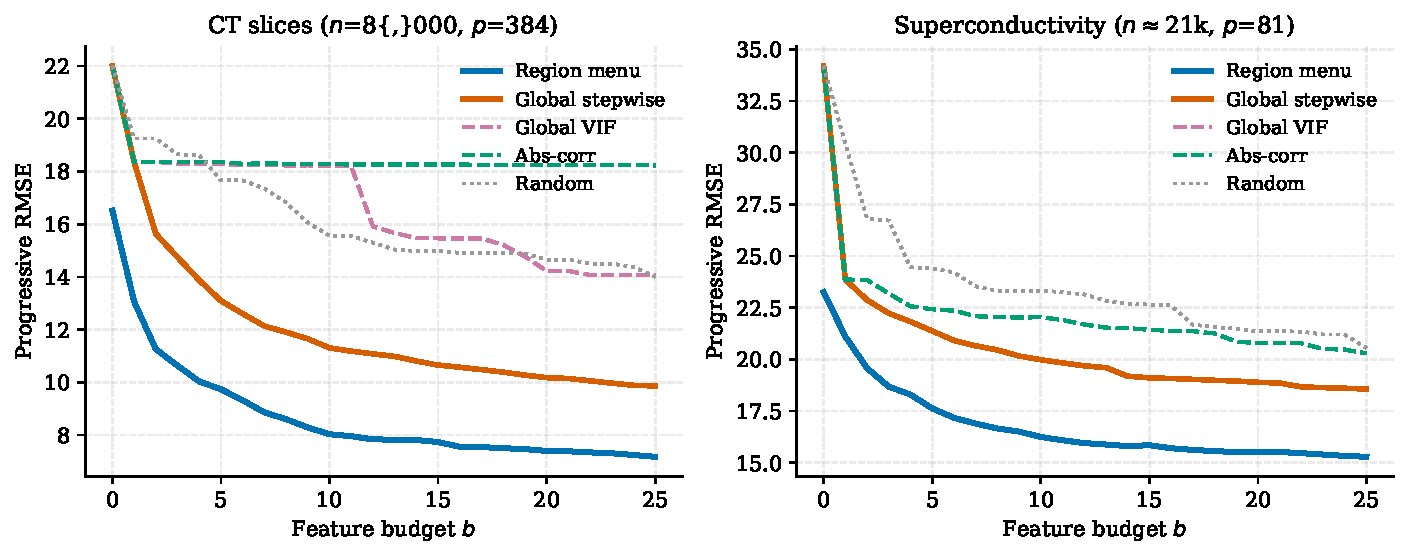
\includegraphics[width=\textwidth]{fig2_progressive_main.pdf}
\caption{Progressive root-mean-square error (RMSE) versus feature budget on computed tomography (CT) slices (\(n=8{,}000\), \(p=384\); \textbf{a}) and superconductivity (\(n\approx 21\text{k}\), \(p=81\); \textbf{b}). Region menus use residual partitioning with soft assignment and forward stepwise Bayesian information criterion (BIC) selection. Line styles distinguish methods independently of colour}
\label{fig:main}
\end{figure}

\begin{table}[t]
\centering
\caption{Progressive root-mean-square error (RMSE) on CT slices: region menus versus global one-region forward stepwise}
\label{tab:ct}
\begin{tabular}{@{}lrrrr@{}}
\toprule
Setting & Budget & Region menu & Global one-region & Relative reduction \\
\midrule
\(n=8{,}000\) & 5 & 9.74 & 13.09 & \(\sim\)26\% \\
\(n=8{,}000\) & 25 & 7.17 & 9.86 & \(\sim\)27\% \\
\(n=20{,}000\) & 5 & 9.63 & 13.14 & \(\sim\)27\% \\
\(n=20{,}000\) & 25 & 7.26 & 10.01 & \(\sim\)28\% \\
\(n=53{,}500\) (train \(\approx 40{,}125\)) & 5 & 9.85 & 13.43 & \(\sim\)27\% \\
\(n=53{,}500\) & 25 & 7.36 & 9.97 & \(\sim\)26\% \\
\bottomrule
\end{tabular}
\end{table}

\begin{figure}[t]
\centering
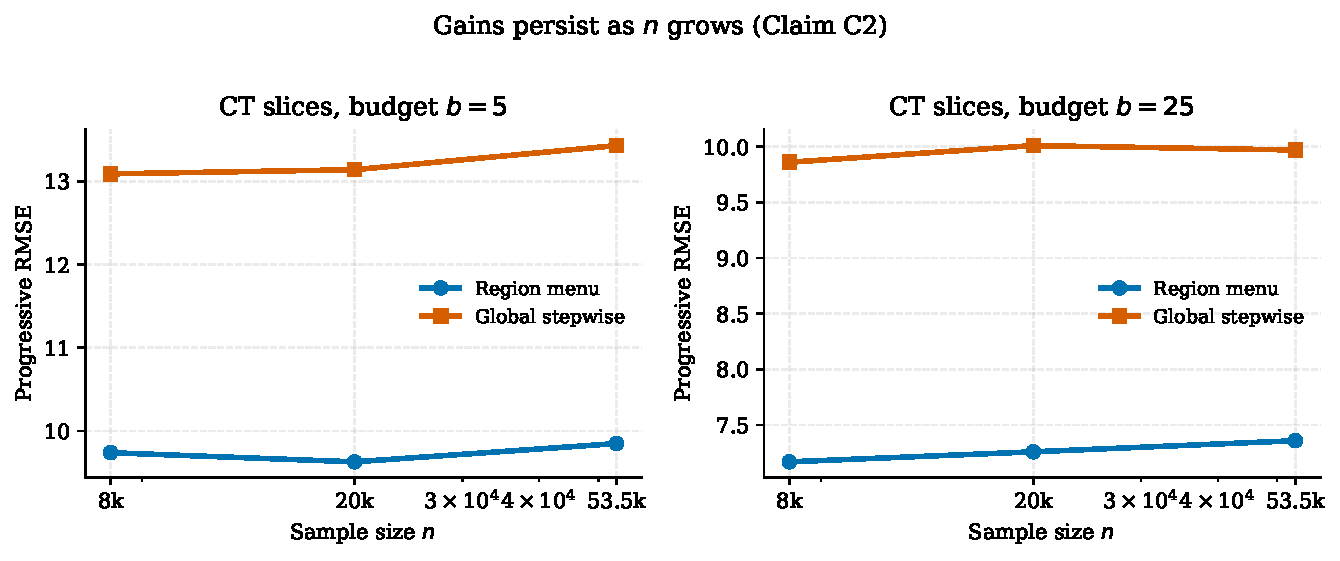
\includegraphics[width=\textwidth]{fig3_ct_scaling.pdf}
\caption{Computed tomography (CT) slice progressive root-mean-square error (RMSE) at fixed budgets as training sample size \(n\) grows. The gap versus global stepwise remains large, supporting Claim~C2}
\label{fig:scaling}
\end{figure}

Two qualitative observations reinforce Table~\ref{tab:ct} and Figs.~\ref{fig:main}--\ref{fig:scaling}. Residual/soft and \(k\)-means/soft variants perform similarly on CT slices, so the gap is not a fragile partition-channel artifact. Relative to abs-corr and random orders in Fig.~\ref{fig:main}, both region and global stepwise are stronger, but region menus widen the lead on the anytime metric.

\subsubsection{Menus as local knowledge}
\label{sec:menu-knowledge}
A trivial explanation of the RMSE gap would be four noisy copies of one ranking. Table~\ref{tab:named} rules that out. On the CT \(n=8{,}000\) split of Fig.~\ref{fig:main}a, mean pairwise Jaccard similarity of the first eight stepwise features is \(0.011\) across regions (sizes \(1651\), \(1765\), \(1741\), \(843\)). On superconductivity it is \(0.057\) (sizes \(7967\), \(3530\), \(2466\), \(1984\)).

UCI CT descriptors are 240 polar-histogram bins of bone structure followed by 144 bins of air inclusions. Region \(r=3\) spends its first six acquisitions on bone bins; region \(r=1\) spends five of six on air-inclusion bins; regions \(r=0\) and \(r=2\) mix the two channels in different orders. Superconductivity features are ten statistics of eight elemental properties, plus the number of elements \cite{hamidieh2018}. Region \(r=0\) leads with thermal conductivity, \(r=1\) with mean atomic mass, \(r=2\) with electron affinity, and \(r=3\) with a mix of ionization energy, affinity, valence, and density. Weighted-mean thermal conductivity (index \(62\)) appears in two prefixes, so a shared transport descriptor can still be acquired early while mass, affinity, and ionization specialize. The menus are local acquisition knowledge, not a restatement of the pooled path.

\begin{table}[t]
\centering
\caption{First six residual/soft menu entries with UCI names (same split as Fig.~\ref{fig:main}). CT: polar-histogram bins. Superconductivity: Hamidieh elemental statistics. Column indices are \(0\)-based}
\label{tab:named}
\small
\begin{tabular}{@{}lp{0.72\textwidth}@{}}
\toprule
Region & First six named acquisitions \\
\midrule
\multicolumn{2}{@{}l}{\emph{CT slices}} \\
\(r=0\) (\(n_r=1651\)) & bone bins \(45,133\); air bin \(24\); bone bins \(3,131,237\) \\
\(r=1\) (\(n_r=1765\)) & air bins \(92,18\); bone bin \(72\); air bins \(66,13,48\) \\
\(r=2\) (\(n_r=1741\)) & bone bin \(4\); air bin \(33\); bone bins \(135,118,180,222\) \\
\(r=3\) (\(n_r=843\)) & bone bins \(215,36,171,95,123,125\) \\
\midrule
\multicolumn{2}{@{}l}{\emph{Superconductivity}} \\
\(r=0\) (\(n_r=7967\)) & weighted mean thermal conductivity; weighted std.\ electron affinity; weighted range / std.\ atomic radius; std.\ atomic mass; mean thermal conductivity \\
\(r=1\) (\(n_r=3530\)) & mean atomic mass; weighted range fusion heat; weighted range thermal conductivity; weighted mean first ionization energy; weighted std.\ fusion heat; weighted std.\ first ionization energy \\
\(r=2\) (\(n_r=2466\)) & mean / weighted mean electron affinity; weighted std.\ atomic mass; weighted mean first ionization energy; weighted geometric mean / std.\ thermal conductivity \\
\(r=3\) (\(n_r=1984\)) & weighted entropy first ionization energy; weighted geometric mean electron affinity; weighted mean thermal conductivity; geometric mean valence; range density; range atomic radius \\
\bottomrule
\end{tabular}
\end{table}

\subsubsection{Localized sparse regression as an anytime neighbor}
\label{sec:lasso-neighbor}
Table~\ref{tab:lasso} compares forward-stepwise region menus with localized Lasso--LARS menus under the same residual/soft partition, nested prefix OLS, splits, and budgets. Regionalization itself helps: Lasso--LARS menus beat global stepwise at the reported budgets. The stepwise constructor remains stronger at early budgets, where acquisition knowledge matters most (CT, budget \(5\): \(9.74\) versus \(12.31\) versus \(13.09\); superconductivity, budget \(5\): \(17.63\) versus \(19.13\) versus \(21.38\)). The gap is smaller at budget \(25\), consistent with Lasso--LARS eventually finding useful supports while remaining a weaker schedule for the first measurements. Thus the contribution is not clustering alone; it is the combination of regional knowledge with a constructor that is scored---and here, better---as an ordered menu.

\begin{table}[t]
\centering
\caption{Anytime RMSE for forward-stepwise region menus, localized Lasso--LARS menus on the same partition, and global one-region stepwise}
\label{tab:lasso}
\begin{tabular}{@{}lrrrr@{}}
\toprule
Dataset & Budget & Region stepwise & Region Lasso--LARS & Global stepwise \\
\midrule
CT slices (\(n=8{,}000\)) & 5 & 9.74 & 12.31 & 13.09 \\
CT slices (\(n=8{,}000\)) & 25 & 7.17 & 8.38 & 9.86 \\
Superconductivity & 5 & 17.63 & 19.13 & 21.38 \\
Superconductivity & 25 & 15.29 & 15.76 & 18.57 \\
\bottomrule
\end{tabular}
\end{table}

\subsubsection{Instance-adaptive greedy acquisition}
\label{sec:lrg}
Claim~C4 asks whether the CT and superconductivity gains could be recovered by letting each query choose the next measurement from a local residual. Table~\ref{tab:lrg} uses the same seed-0 splits as Tables~\ref{tab:ct}--\ref{tab:lasso}. LRG matches global stepwise at \(b=1\) by construction, then fans out across queries, yet it is weaker than pooled stepwise at later budgets and substantially weaker than region menus (CT, \(b=5\): \(9.74\) versus \(13.09\) versus \(13.40\)). Neighbourhood residual-greedy adds path diversity without useful early-acquisition knowledge: local RSS on \(k=80\) neighbours is noisier than a global stepwise path, whereas four inspectable menus remain the better schedule.

\begin{table}[t]
\centering
\caption{Anytime RMSE for region menus, global one-region stepwise, and local residual-greedy (LRG) instance-adaptive acquisition. LRG matches global stepwise at budget \(1\) and then diverges across queries}
\label{tab:lrg}
\begin{tabular}{@{}lrrrr@{}}
\toprule
Dataset & Budget & Region menu & Global stepwise & LRG \\
\midrule
CT slices (\(n=8{,}000\)) & 1 & 13.07 & 18.37 & 18.37 \\
CT slices (\(n=8{,}000\)) & 5 & 9.74 & 13.09 & 13.40 \\
CT slices (\(n=8{,}000\)) & 13 & 7.82 & 10.98 & 11.46 \\
CT slices (\(n=8{,}000\)) & 25 & 7.17 & 9.86 & 10.86 \\
Superconductivity & 1 & 21.10 & 23.86 & 23.86 \\
Superconductivity & 5 & 17.63 & 21.38 & 21.92 \\
Superconductivity & 13 & 15.88 & 19.60 & 20.92 \\
Superconductivity & 25 & 15.29 & 18.57 & 19.81 \\
\bottomrule
\end{tabular}
\end{table}

\subsubsection{Measurement budget as a decision-support reading}
\label{sec:budget-ds}
Fig.~\ref{fig:budget} rereads the CT and superconductivity curves as the smallest \(b\) at which a region menu matches global stepwise error at a stated operating point. On the seed-0 splits, that match to global \(b=5\) occurs after one measurement on both tasks, and the match to global \(b=25\) after five measurements on CT slices and four on superconductivity. Across repeated splits the means are \(1.6\) and \(1.7\) to match global \(b=5\), and \(4.6\) and \(4.0\) to match global \(b=25\).

\begin{figure}[t]
\centering
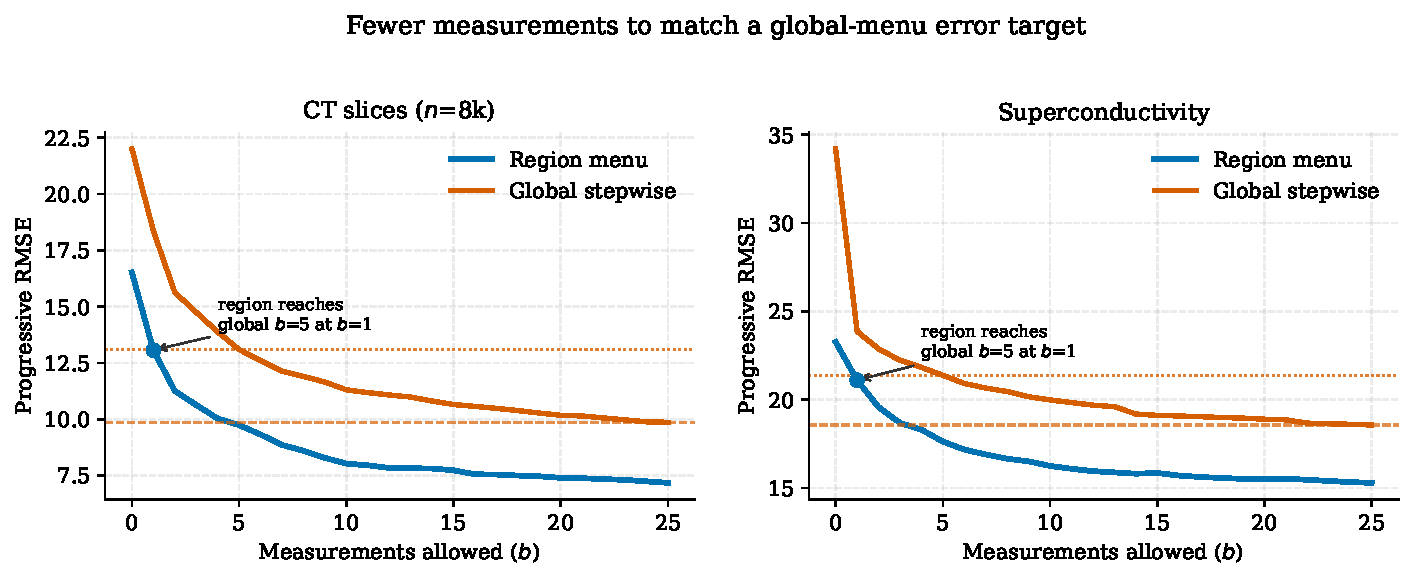
\includegraphics[width=\textwidth]{fig6_measurement_budget.pdf}
\caption{Progressive RMSE versus number of allowed measurements. Horizontal dotted and dashed guides mark global stepwise error at budgets \(b=5\) and \(b=25\), respectively. Markers indicate the first regional budget that matches the global \(b=5\) target. Panels: \textbf{a} CT slices; \textbf{b} superconductivity}
\label{fig:budget}
\end{figure}

\subsubsection{Stability of the mined knowledge}
\label{sec:stability}
Menus are knowledge only if they do not dissolve under a change of train/test split. Table~\ref{tab:stability} reports pairwise Jaccard similarity of (i)~the covering set of the first eight features from all regions and (ii)~the global stepwise top-eight list, together with how many features appear in at least half of the covering sets. Global top-eight lists are more stable, as expected for a single pooled ranking. Regional covering sets still overlap substantially (mean Jaccard \(0.53\) on CT slices over five splits; \(0.46\) on superconductivity over ten splits), and \(30\) (CT) and \(26\) (superconductivity) features recur in at least half of the splits. The anytime advantage itself is stable: region RMSE at \(b=5\) remains in a narrow band (about \(9.2\)--\(10.1\) on CT; \(17.4\)--\(17.9\) on superconductivity) and stays below the corresponding global values on every split. Regional knowledge is therefore noisier than one global list---there are more degrees of freedom---but it is not an artifact of a single partition of the data.

\begin{table}[t]
\centering
\caption{Stability of early-feature knowledge across random train/test splits. Covering set: union of the first eight features of all regional menus. Jaccard is the mean pairwise similarity of those sets (or of global top-eight lists)}
\label{tab:stability}
\small
\begin{tabular}{@{}lcccc@{}}
\toprule
Dataset & Splits & Jaccard (region) & Jaccard (global) & Recurring features \\
\midrule
CT slices (\(n=8\)k) & 5 & 0.53 & 0.77 & 30 \\
Superconductivity & 10 & 0.46 & 0.66 & 26 \\
\bottomrule
\end{tabular}
\end{table}

\subsection{Results on superconductivity}
\label{sec:sc}

\textbf{Claim.} On superconductivity critical-temperature prediction, region menus again improve progressive RMSE against global stepwise, abs-corr, and VIF, supporting C1 beyond a single application domain.

The progressive RMSE curves on superconductivity are shown in Fig.~\ref{fig:main}b, and selected budgets are reported in Table~\ref{tab:sc}. Region menus improve progressive RMSE against global stepwise and abs-corr across budgets. Table~\ref{tab:lrg} shows the same split for LRG, supporting C1 and C4 jointly. Named prefixes in Table~\ref{tab:named} already record the shared thermal-conductivity / ionization-energy descriptors and the region-specific mass, fusion-heat, and affinity entries.

\begin{table}[t]
\centering
\caption{Progressive root-mean-square error (RMSE) on superconductivity}
\label{tab:sc}
\begin{tabular}{@{}rrrr@{}}
\toprule
Budget & Region (best) & Global one-region & Abs-corr (approx.) \\
\midrule
5 & 17.63 & 21.38 & 22.43 \\
13 & 15.88 & 19.60 & 21.54 \\
25 & 15.29 & 18.57 & 20.30 \\
\bottomrule
\end{tabular}
\end{table}

\subsection{Results on tecator spectra}
\label{sec:tecator}

\textbf{Claim.} Under scarce samples relative to dimensionality, regional menus can still improve early- and mid-budget error relative to a pooled stepwise menu, provided regions remain adequately populated.

On tecator (\(n=240\), \(p=124\)), region menus achieve approximately 0.77 RMSE at budget 5 versus approximately 1.18 for global one-region stepwise, with the advantage continuing at several higher budgets (e.g., final reported budgets near 0.75 vs.\ 0.88). These reported budget comparisons are summarized as bars in Fig.~\ref{fig:mixed}b. This matters scientifically because fragmentation risk is highest precisely in the high-\(p\)/low-\(n\) regime. The result suggests that bias reduction from local relevance can outweigh variance inflation from splitting, at least when stepwise BIC prevents aggressive over-selection.

\subsection{Mixed results on hard synthetics}
\label{sec:synth}

\textbf{Claim (bounded).} Regional menus are not guaranteed to beat a strong global stepwise path merely because local supports differ in the generative model.

On the hard synthetics described in Section~\ref{sec:datasets} (\(p\in\{1000,2000\}\); three regions with planted 15-feature supports and correlated covariates), region menus beat random and abs-corr baselines and often beat global VIF, yet global one-region forward stepwise frequently attains the best high-budget RMSE (e.g., \(p=2000\), budget 25: global \(\approx 10.12\) vs.\ region \(\approx 10.47\)--\(10.50\)). A representative progressive curve for \(p=1000\) is shown in Fig.~\ref{fig:mixed}a: at very small budgets the comparison is closer and sometimes favors regions, but the anytime curve does not uniformly dominate.

\begin{figure}[t]
\centering
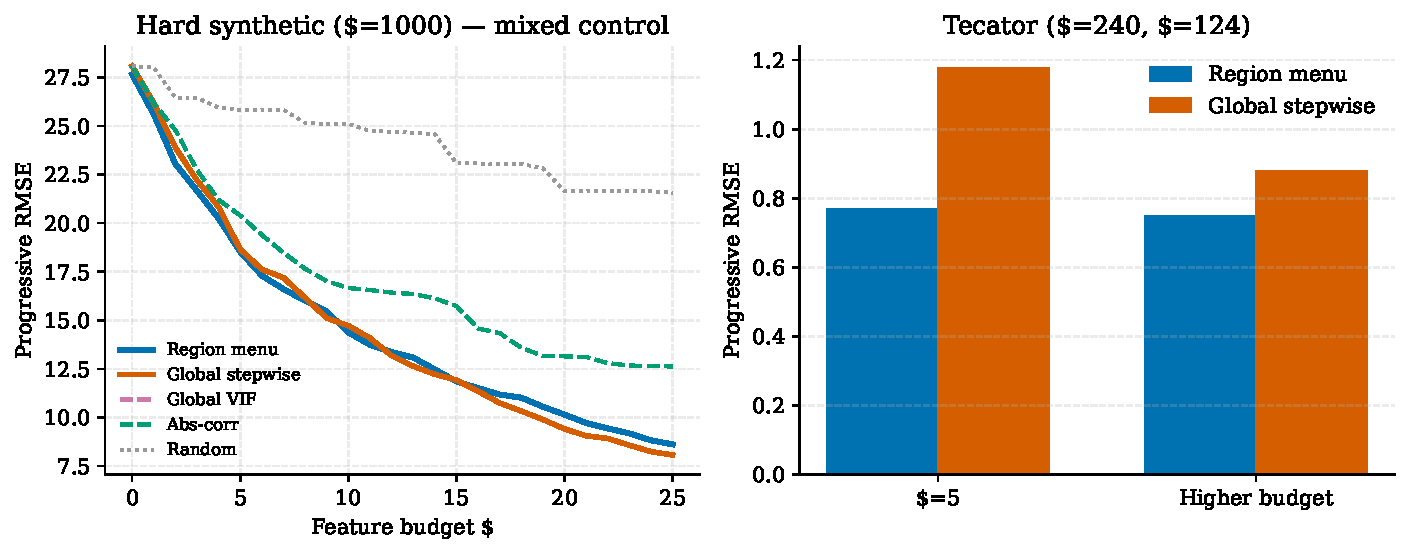
\includegraphics[width=\textwidth]{fig4_mixed_and_tecator.pdf}
\caption{\textbf{a} Progressive root-mean-square error (RMSE) on a hard correlated synthetic (\(p=1000\)), where global stepwise can remain competitive at higher budgets (Claim~C3). \textbf{b} tecator RMSE at reported budgets for region menus versus global stepwise}
\label{fig:mixed}
\end{figure}

This mixed outcome is informative rather than fatal. Pooled stepwise can still surface a useful union of supports when signals are strong and regions are linearly separable in only a few coordinates. Soft assignment and finite per-region samples can further blunt specialization. Hence C1 requires empirical heterogeneity that harms global early acquisition, not only planted differences in support sets.

\subsection{Weak-signal control}
\label{sec:topo}

\textbf{Claim (negative control).} When covariates carry little usable linear signal, progressive policies cannot manufacture accuracy; regional menus neither help nor hurt in a meaningful way.

On topo\_2\_1 (\(n\approx 8.9\times 10^3\), \(p=266\)), RMSE values remain nearly flat across methods (\(\approx 0.027\)--\(0.029\)). This validates C3: anytime curves must be read conditionally on the existence of predictable structure. Including such a control protects the paper against the criticism that regional menus always look better under any high-\(p\) regime.

\subsection{When to regionalize}
\label{sec:when}
\textbf{Claim.} The mixed controls in Sections~\ref{sec:synth}--\ref{sec:topo} can be turned into an operational pre-test rather than only a verbal caveat.

Table~\ref{tab:when} reports the inner-validation rule of Section~\ref{sec:method-pretest} on three random splits per dataset. On CT slices (\(n=8{,}000\)), superconductivity, and tecator, the rule selects the regional policy on every split, matching the test-set winner at \(b=5\). On a correlated synthetic with planted regional supports (\(p=80\)), where pooled stepwise is already better at mid-budgets, the same rule selects the global menu on every split. Mean test RMSE at \(b=5\) for the chosen policy therefore coincides with the oracle that peeks at the test fold. Mean pairwise Jaccard overlap of the first five regional features is not a reliable surrogate, nor is training BIC of the prefix mixture. The recommended rule is the nested RMSE comparison. On topo\_2\_1 the two test curves differ only in the fourth decimal place, so either policy is acceptable.

\begin{table}[t]
\centering
\caption{Train-only choice of regional versus global menus at budget \(b=5\). Inner validation uses 20\% of the training fold. Test RMSE is after refitting the selected policy on the full training fold}
\label{tab:when}
\small
\begin{tabularx}{\textwidth}{@{}>{\raggedright\arraybackslash}Xcccccc@{}}
\toprule
 & & \multicolumn{2}{c}{Policy} & \multicolumn{3}{c}{Test RMSE at \(b=5\)} \\
\cmidrule(lr){3-4}\cmidrule(lr){5-7}
Dataset & Splits & Val. & Oracle & Chosen & Region & Global \\
\midrule
Synthetic \(p=80\) & 3 & global & global & 7.11 & 7.89 & 7.11 \\
CT slices (\(n=8\)k) & 3 & region & region & 9.61 & 9.61 & 13.03 \\
Superconductivity & 3 & region & region & 17.49 & 17.49 & 20.95 \\
Tecator & 3 & region & region & 0.91 & 0.91 & 1.27 \\
topo\_2\_1 & 3 & mixed & tied & 0.027 & 0.027 & 0.027 \\
\bottomrule
\end{tabularx}
\end{table}

\subsection{Summary of empirical findings}
\label{sec:summary}

Taken together, heterogeneous real tasks support C1--C2 and C4: region menus improve anytime RMSE, scale with \(n\) on CT slices, match global error with fewer measurements (Fig.~\ref{fig:budget}), and beat both localized Lasso--LARS and LRG at early budgets. Table~\ref{tab:named} shows that the menus are named, region-specific knowledge. Table~\ref{tab:when} and Fig.~\ref{fig:rel} support C3 and C5: a nested RMSE check deploys regional menus on the wins and a global menu on the mixed synthetic, while topo\_2\_1 remains a flat negative control.

\begin{figure}[t]
\centering
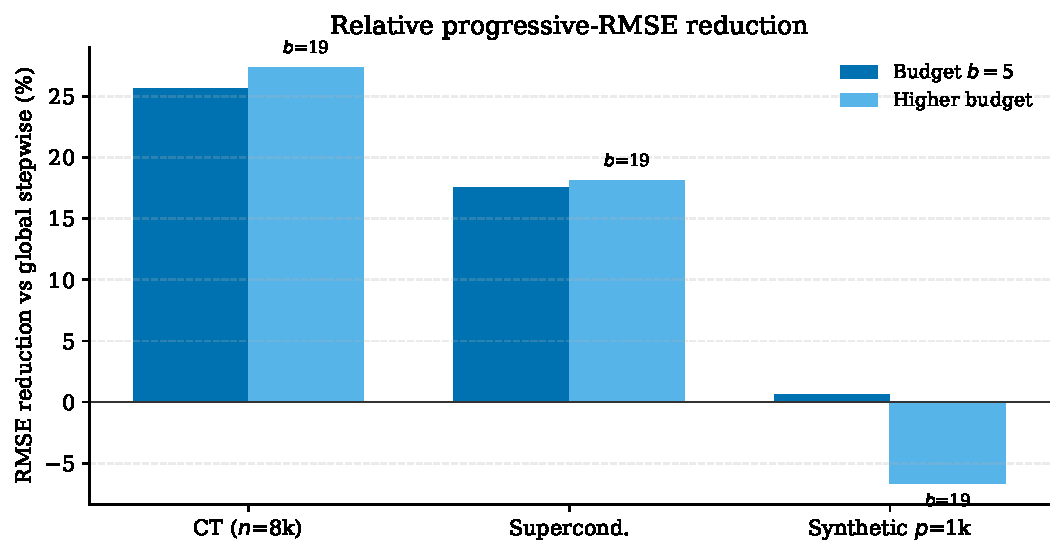
\includegraphics[width=0.72\textwidth]{fig5_relative_reduction.pdf}
\caption{Relative progressive root-mean-square error (RMSE) reduction of region menus versus global stepwise at budget~$b=5$ and at a higher budget. Positive values favor region menus; the synthetic control shows limited or reversed gains at higher budgets}
\label{fig:rel}
\end{figure}

\section{Discussion}
\label{sec:discussion}

The decisive quantity is early-budget risk, equivalently how many measurements are needed to reach a usable error. Global orders blur subgroup-specific relevance. On CT slices and superconductivity that delay is large (often \(\sim\)25\% RMSE on CT at \(b=5\); Table~\ref{tab:ct}) and the same error target is reached with several times fewer features (Fig.~\ref{fig:budget}). The gap persists as \(n\) grows (Fig.~\ref{fig:scaling}), so it is not a small-sample artifact.

Regional menus are not a free improvement for every high-\(p\) problem (Fig.~\ref{fig:mixed}a; Fig.~\ref{fig:rel}). They are most justified when (i) predictive mechanisms differ across regions of \(\mathbf{X}\), (ii) those differences affect which features should be acquired early, and (iii) each region has enough samples for stable stepwise selection. If (i)--(ii) fail, one global menu is often enough; if signal fails, no ordering policy matters. Section~\ref{sec:when} shows that this scope can be checked from training data by inner-validation RMSE at a small budget.

Table~\ref{tab:lrg} shows that coarseness relative to a fully dynamic acquisition policy \cite{ma2019,covert2023} is not a handicap on the heterogeneous tasks: LRG, which already adapts the next coordinate to observed values, remains worse than global stepwise and far worse than regional menus. Piecewise-constant menus are therefore a strong inspectable baseline, not a substitute for a full acquisition MDP.

\textbf{Limitations.} Partitioning is heuristic and is not jointly optimized with menu learning. Soft-assignment temperature and the residual weight are held fixed; \(R\) and \(m_{\max}\) follow \(n\)/\(p\) rules, and the pre-test chooses only between that \(R\) and \(R=1\). Prefix models are linear. Regional covering sets are less stable than a global top-eight list (Table~\ref{tab:stability}), while the anytime advantage is stable across splits.

\section{Conclusion}
\label{sec:conclusion}

Progressive feature revelation reframes feature selection as the design of acquisition knowledge: predictions must be accurate before all covariates are known. Region-specific incremental feature menus were introduced as a practical representation for that setting. Through partitioning of the input space and construction of per-region forward-stepwise menus with nested prefix models, acquisition order is adapted to local relevance while remaining statistically transparent and computationally scalable.

The empirical message is bounded. On CT-slice localization and superconductivity, regional menus improve progressive RMSE, survive large \(n\), reach the same error with fewer measurements, remain advantageous across splits, and beat localized Lasso--LARS and local residual-greedy acquisition at early budgets. Named prefixes distinguish bone versus air histogram channels on CT slices and elemental-property families on superconductivity. On weak-signal data and some correlated synthetics a global stepwise menu remains competitive; a nested RMSE check at budget \(5\) recovers that condition from training data. Region-specific menus are therefore inspectable local acquisition knowledge for anytime regression under partial observation, and a baseline against which heavier dynamic acquisition methods should be compared.

\backmatter

\section*{Statements and Declarations}

\subsection*{Competing interests}
The author has no relevant financial or non-financial interests to disclose.

\subsection*{Funding}
The author declares that no funds, grants, or other support were received during the preparation of this manuscript.

\subsection*{Author contributions}
Hoa Dinh Nguyen designed the study, implemented the method, ran the experiments, and wrote the manuscript.

\subsection*{Ethics approval}
Not applicable.

\subsection*{Consent to participate}
Not applicable.

\subsection*{Consent for publication}
Not applicable.

\subsection*{Data and code availability}
The datasets analyzed in this study are publicly available:
\begin{itemize}
  \item Relative location of CT slices on axial axis (UCI Machine Learning Repository): \url{https://archive.ics.uci.edu/dataset/206/relative+location+of+ct+slices+on+axial+axis}
  \item Superconductivity data (UCI Machine Learning Repository): \url{https://archive.ics.uci.edu/dataset/464/superconductivty+data}
  \item Tecator (OpenML): \url{https://www.openml.org/d/505}
  \item topo\_2\_1 (OpenML): \url{https://www.openml.org/search?type=data&name=topo_2_1}
\end{itemize}
Synthetic data can be regenerated with the accompanying experiment scripts. Source code is available at \url{https://github.com/dinhhoaptit/region-specific-feature-menus} (\texttt{src/} and \texttt{examples/}; see \texttt{README.md}).

\bibliography{references}

\end{document}

